\chapter{Medições em Laboratório}

A segunda etapa desta prática consistiu na montagem física dos circuitos projetados e na aquisição empírica de seus dados de resposta em frequência. O objetivo primordial desta fase é levantar os dados reais de bancada para o traçado do diagrama de Bode e confrontá-los com as previsões matemáticas oriundas da análise teórica, avaliando os impactos das tolerâncias dos componentes e das não-idealidades do amplificador operacional comercial.

A infraestrutura de instrumentação utilizada na bancada compreendeu:
\begin{itemize}
	\item Fonte de tensão contínua simétrica, ajustada para fornecer a alimentação de $\pm 10\text{ V}$ ao amplificador operacional;
	\item Gerador de funções arbitrário, empregado para injetar o sinal senoidal de excitação ($v_i(t)$) no circuito;
	\item Osciloscópio digital de múltiplos canais para monitoramento simultâneo do sinal de entrada (Canal 1) e da resposta do filtro (Canal 2);
	\item Multímetro digital de bancada para a aferição dos valores reais dos componentes passivos antes da inserção no circuito.
\end{itemize}

\section{Circuito 1: Filtro Passa-Baixa Superamortecido}

\subsection{Aferição a Frio dos Componentes Passivos}

Para garantir a acurácia da análise comparativa pós-laboratorial, o procedimento inicial consistiu na medição individual da resistência e da capacitância reais dos componentes a serem utilizados. A quantificação exata destes parâmetros permite recalcular a função de transferência do filtro com os valores reais, isolando o erro instrumental do erro provocado pela tolerância de fabricação. A Tabela \ref{tab:componentes_c1} apresenta os valores nominais do projeto mecânico contrastados com as medições efetivas do multímetro.

\begin{table}[H]
	\centering
	\caption{Comparativo entre os valores nominais e medidos dos componentes - Circuito 1.}
	\label{tab:componentes_c1}
	\renewcommand{\arraystretch}{1.2}
	\begin{tabular}{ccc}
		\hline
		\textbf{Componente} & \textbf{Valor Nominal} & \textbf{Valor Medido Experimentalmente} \\ \hline
		Resistor $R_1$ & $47,0\text{ k}\Omega$ & $47,13\text{ k}\Omega$ \\
		Resistor $R_2$ & $470,0\text{ k}\Omega$ & $469,4\text{ k}\Omega$ \\
		Resistor $R_3$ & $470,0\text{ k}\Omega$ & $478,0\text{ k}\Omega$ \\
		Capacitor $C_1$ & $100,0\text{ nF}$ & $109,9\text{ nF}$ \\
		Capacitor $C_2$ & $10,0\text{ nF}$ & $11,42\text{ nF}$ \\ \hline
	\end{tabular}
\end{table}

\subsection{Determinação Prática da Frequência de Corte ($f_1$)}

Após a montagem do circuito em matriz de contatos (\textit{protoboard}), iniciou-se a busca pela frequência de corte de $-3\text{ dB}$, denotada por $f_1$. Para um filtro passa-baixa, esta frequência corresponde ao ponto em que a magnitude da tensão de saída decai para aproximadamente $70,7\%$ (ou $1/\sqrt{2}$) do valor de máxima amplitude encontrado nas faixas de frequências mais baixas.

O gerador de sinais foi configurado para varrer a entrada com um sinal senoidal. Em baixas frequências (na região de $1,6\text{ Hz}$), observou-se que a amplitude máxima estabilizada da saída era de $1,04\text{ V}$. 

Tendo como base o ganho máximo no patamar de corrente contínua, o critério de $-3\text{ dB}$ foi calculado como:
\begin{equation}
	V_{o(-3\text{dB})} = V_{o(max)} \times \frac{1}{\sqrt{2}} = 1,04\text{ V} \times 0,7071 \approx 735\text{ mV}
\end{equation}

Aumentando gradativamente a frequência do gerador de funções e observando a atenuação correspondente no Canal 2 do osciloscópio, o limite de $\approx 730\text{ mV}$ na saída foi atingido experimentalmente na marca de \textbf{$4,3\text{ Hz}$}. Este valor foi assumido como a frequência de corte $f_1$ real do circuito montado.

\subsection{Varredura de Frequência e Aquisição de Dados}

Com a frequência de referência $f_1 = 4,3\text{ Hz}$ determinada empiricamente, executou-se uma varredura sistêmica aplicando multiplicadores pré-definidos ao valor de $f_1$ (desde $0,15\times$ até $10\times$). Em cada novo degrau de frequência, registraram-se as amplitudes de pico a pico da excitação ($V_{in}$) e da resposta ($V_{out}$), a fim de levantar os pontos fundamentais para o traçado empírico do diagrama de Bode. 

Os dados resultantes desta varredura estão dispostos na Tabela \ref{tab:varredura_c1}. Nota-se que o ganho sofre uma queda acentuada conforme a frequência se distancia de $f_1$ em direção à banda de rejeição, comportamento que corrobora a característica passa-baixa atenuadora do circuito.

\begin{table}[H]
	\centering
	\caption{Dados experimentais de varredura de frequência para o Primeiro Circuito ($f_1 = 4,3\text{ Hz}$).}
	\label{tab:varredura_c1}
	\renewcommand{\arraystretch}{1.2}
	\begin{tabular}{cccc}
		\hline
		\textbf{Multiplicador} & \textbf{\textflorin  Calculada/Aplicada} & \textbf{Tensão de Entrada ($V_{in}$)} & \textbf{Tensão de Saída ($V_{out}$)} \\ \hline
		$0,15 \times f_1$ & $0,6\text{ Hz}$ & $78\text{ mV}$ & $750\text{ mV}$ \\
		$0,4 \times f_1$ & $1,7\text{ Hz}$ & $132\text{ mV}$ & $1,05\text{ V}$ \\
		$0,6 \times f_1$ & $2,5\text{ Hz}$ & $143\text{ mV}$ & $960\text{ mV}$ \\
		$1,0 \times f_1$ & $4,3\text{ Hz}$ ($f_1$) & $152\text{ mV}$ & $730\text{ mV}$ \\
		$1,2 \times f_1$ & $5,2\text{ Hz}$ & $153\text{ mV}$ & $640\text{ mV}$ \\
		$1,4 \times f_1$ & $6,0\text{ Hz}$ & $153\text{ mV}$ & $570\text{ mV}$ \\
		$1,8 \times f_1$ & $7,7\text{ Hz}$ & $154\text{ mV}$ & $460\text{ mV}$ \\
		$2,5 \times f_1$ & $10,8\text{ Hz}$ & $154\text{ mV}$ & $340\text{ mV}$ \\
		$4,0 \times f_1$ & $17,2\text{ Hz}$ & $155\text{ mV}$ & $210\text{ mV}$ \\
		$6,0 \times f_1$ & $25,8\text{ Hz}$ & $155\text{ mV}$ & $140\text{ mV}$ \\
		$10,0 \times f_1$ & $43,0\text{ Hz}$ & $155\text{ mV}$ & $60\text{ mV}$ \\ \hline
	\end{tabular}
\end{table}

\subsection{Registro Fotográfico e Diagramático}

Para evidenciar a conformidade da montagem com o projeto elétrico e ratificar as grandezas coletadas na Tabela \ref{tab:varredura_c1}, apresenta-se a seguir o registro visual do setup de bancada e as capturas de tela pertinentes extraídas diretamente do osciloscópio durante os ensaios do Circuito 1.

% Grid 1: Fotos da Montagem Física
\begin{figure}[H]
	\centering
	\begin{minipage}{0.45\textwidth}
		\centering
		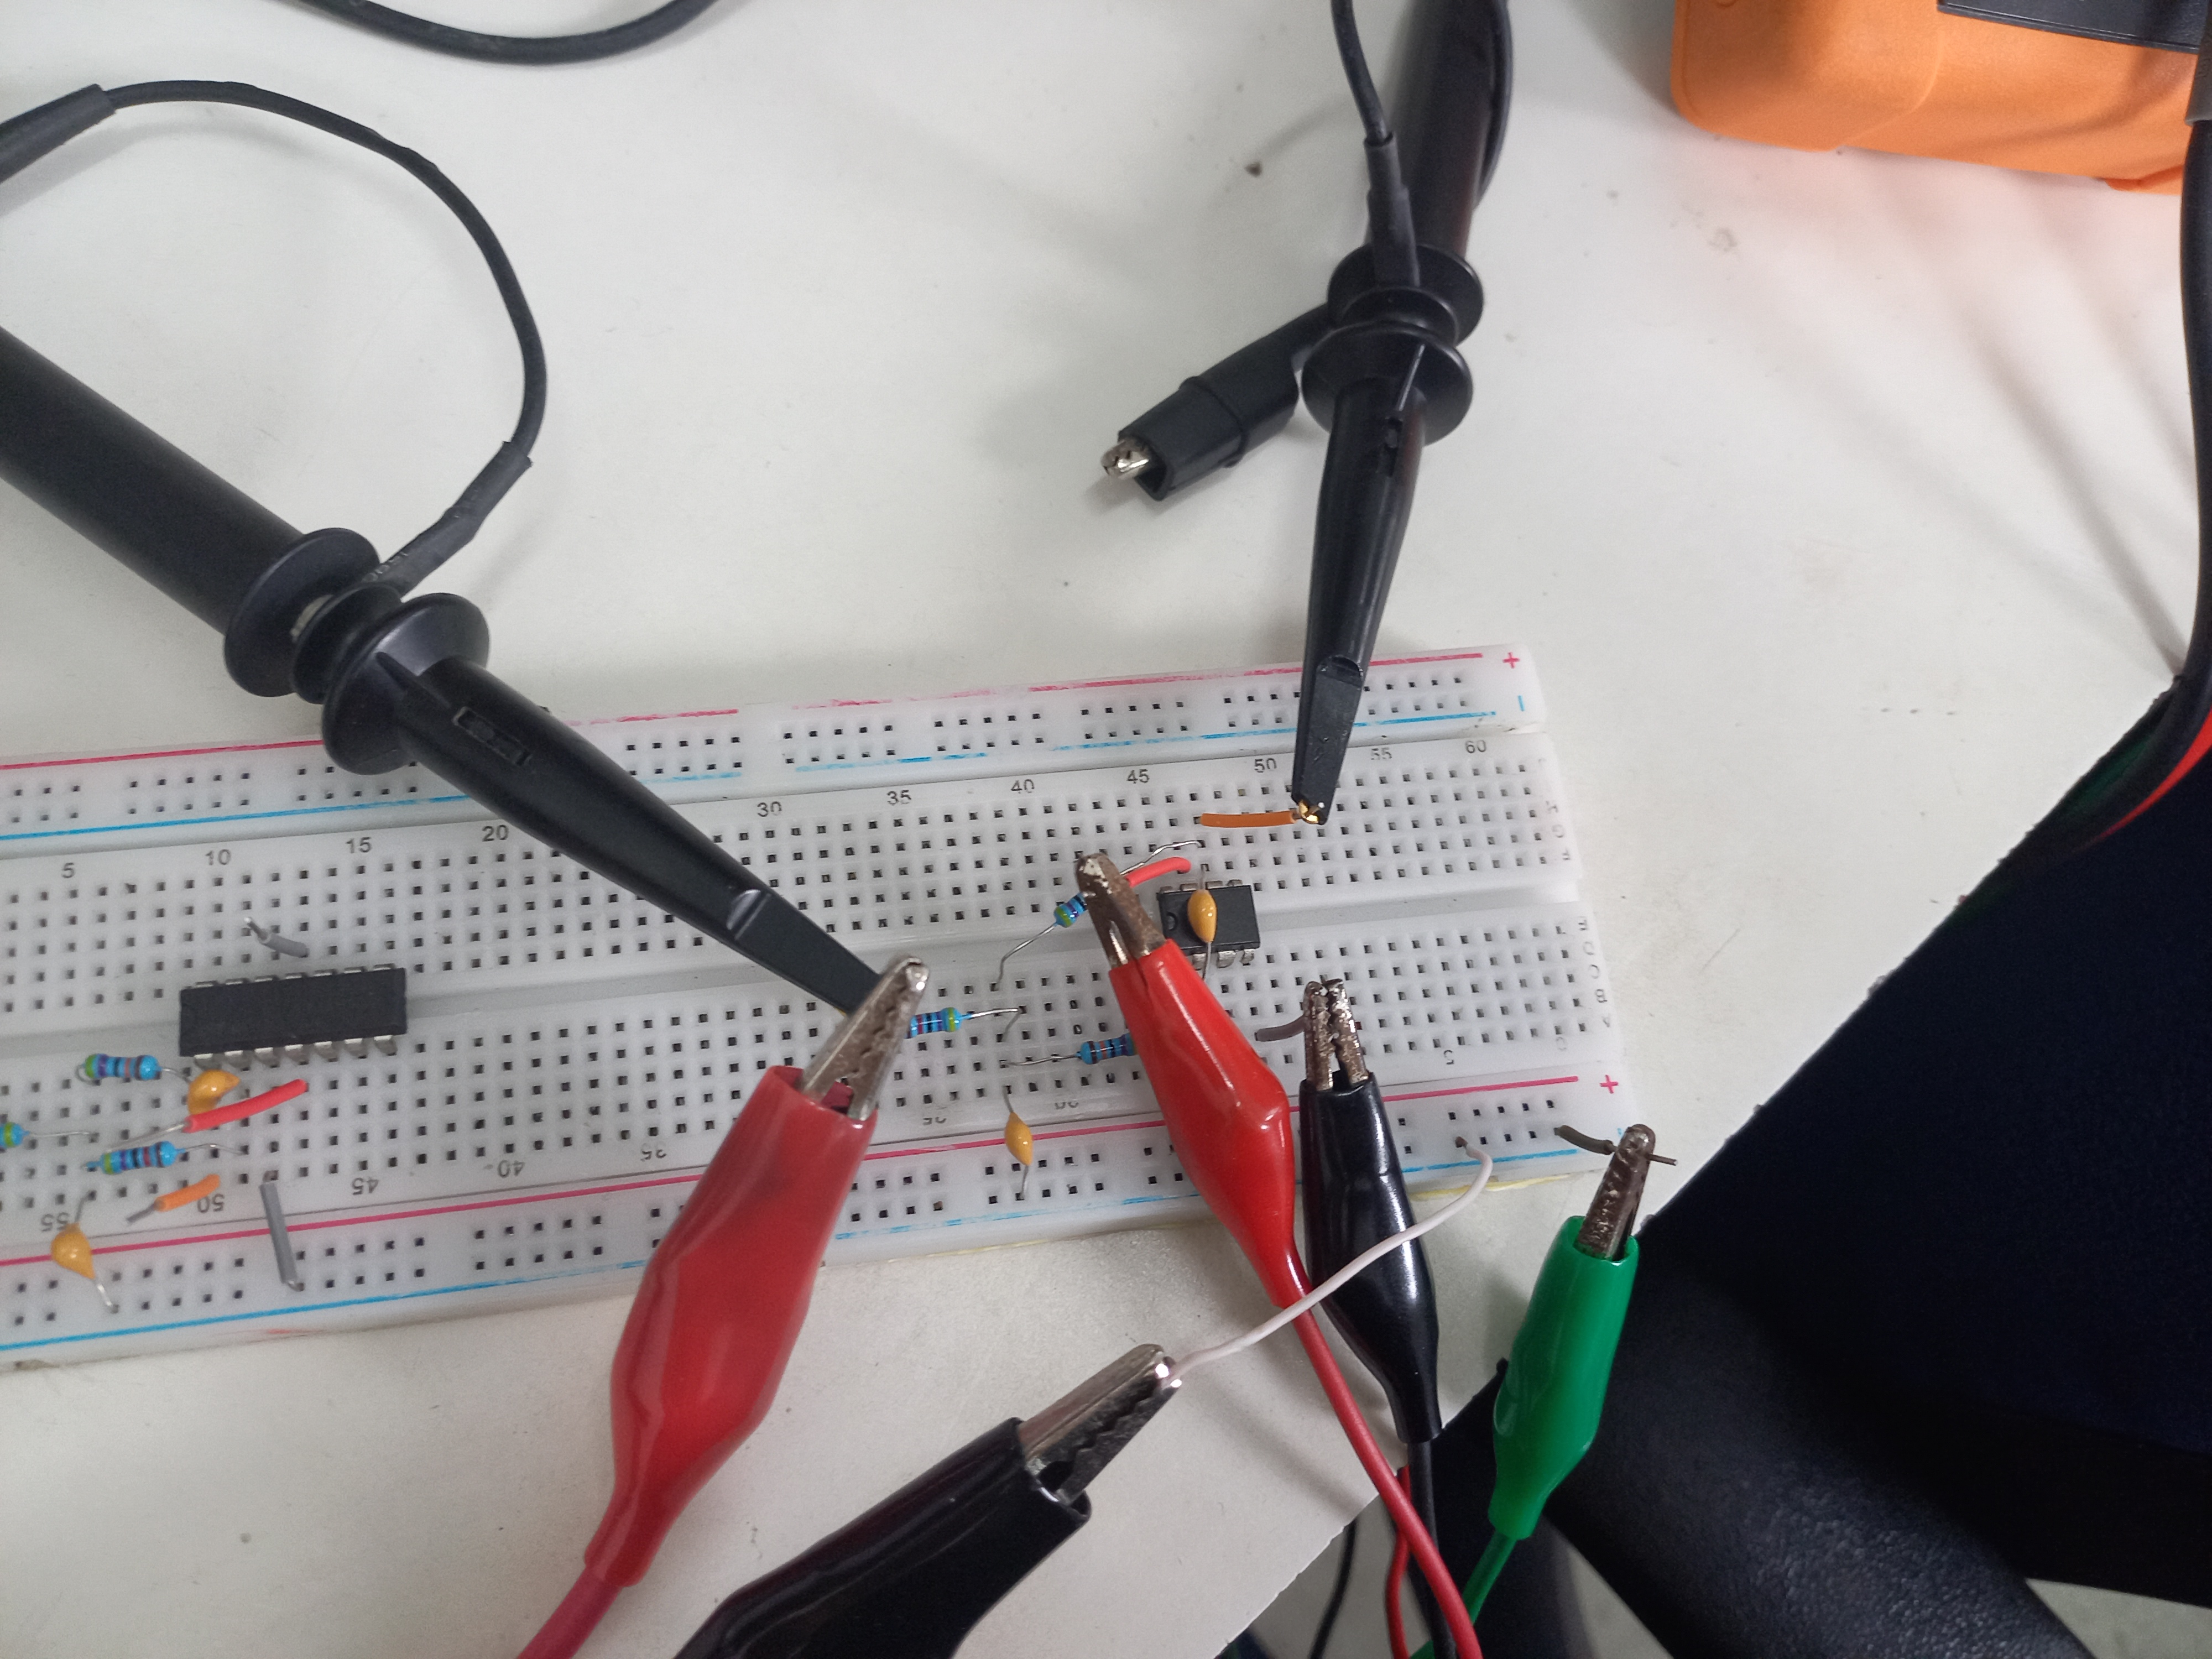
\includegraphics[width=\textwidth]{FIGURAS/circuito_1_montado.jpg}
		\caption{Vista lateral da montagem do Circuito 1 na \textit{protoboard}.}
		\label{fig:c1_montado_1}
	\end{minipage}\hfill
	\begin{minipage}{0.45\textwidth}
		\centering
		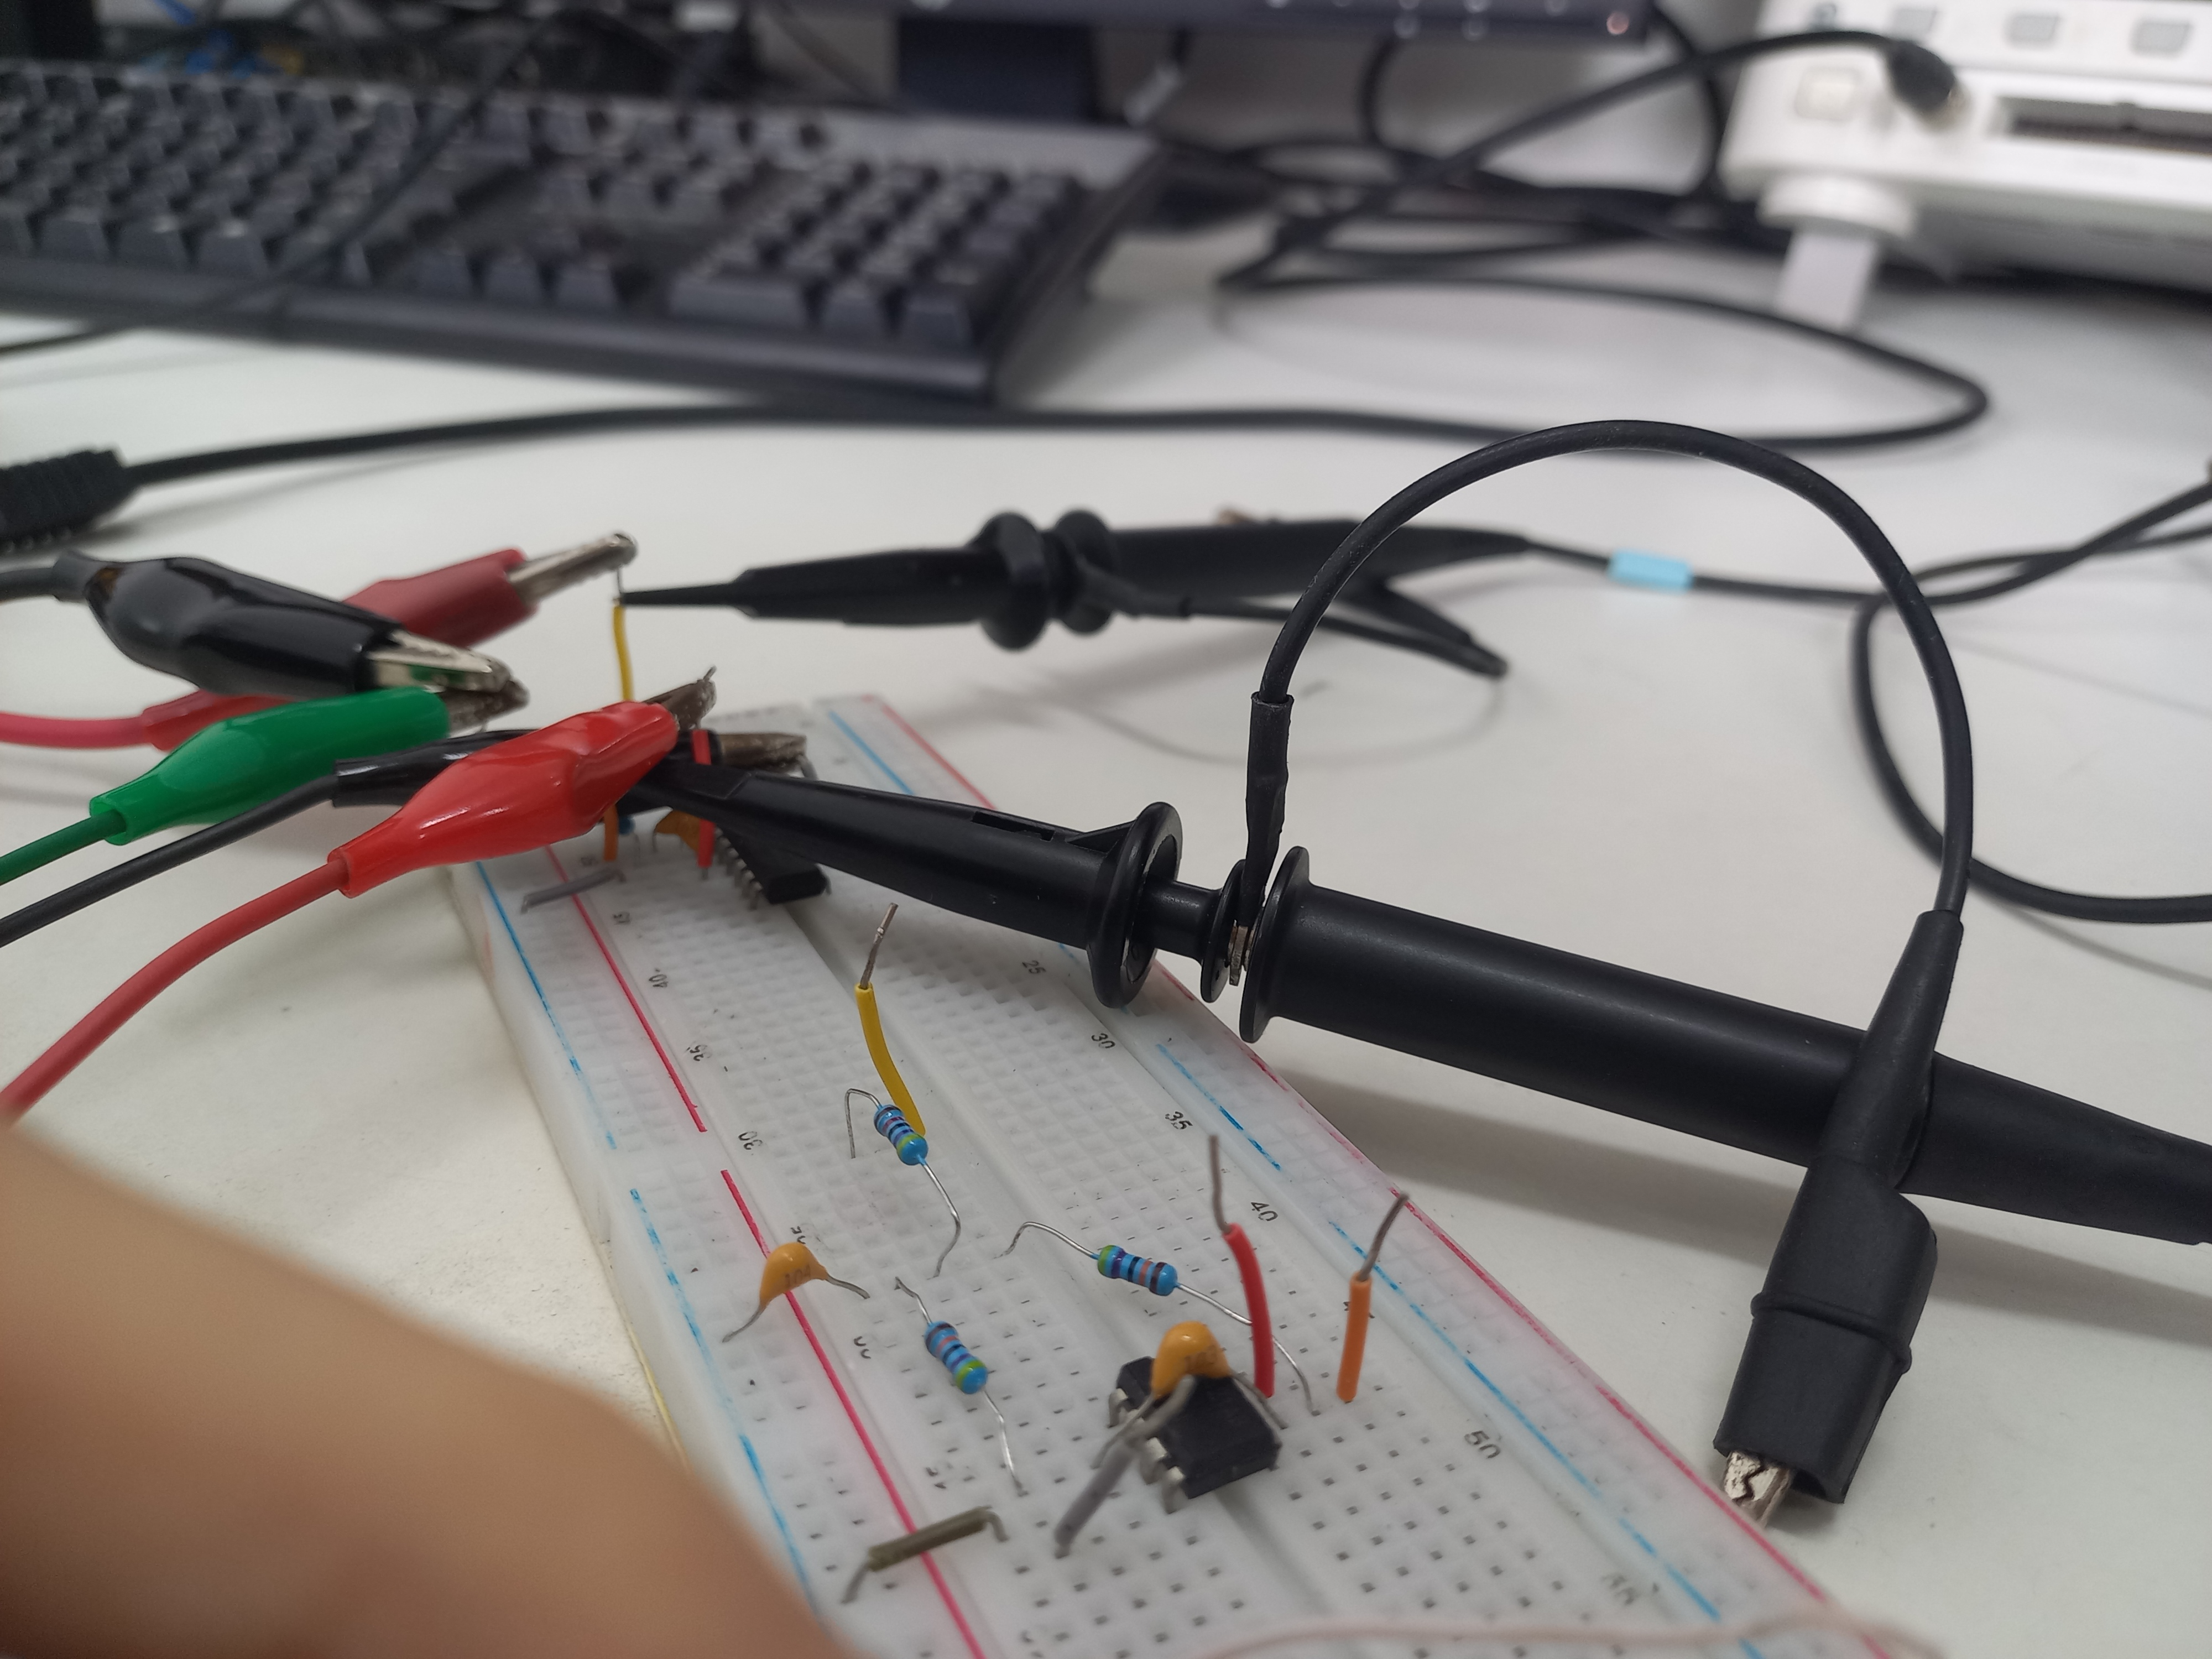
\includegraphics[width=\textwidth]{FIGURAS/circuito_1_montado2.jpg} 
		\caption{Vista superior detalhando o posicionamento do ampop e dos capacitores de poliéster.}
		\label{fig:c1_montado_2}
	\end{minipage}
\end{figure}

% Grid 2: Osciloscópio - Baixas Frequências e f1
\begin{figure}[H]
	\centering
	\begin{minipage}{0.45\textwidth}
		\centering
		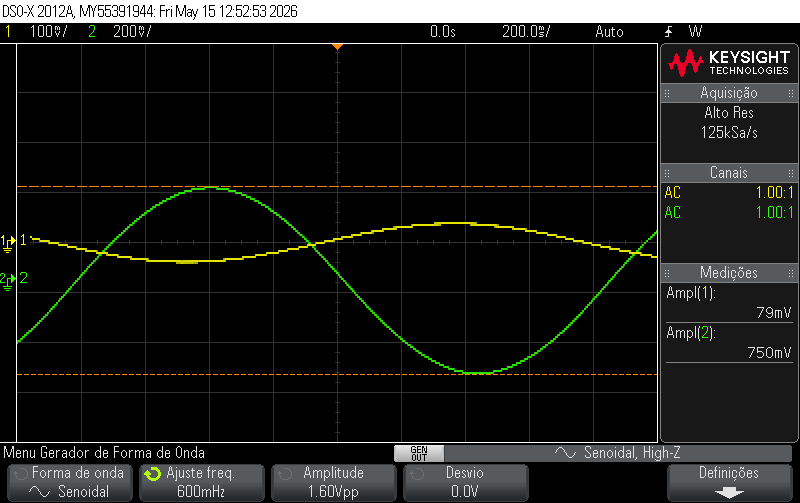
\includegraphics[width=\textwidth]{FIGURAS/600mHz_1.png} 
		\caption{Sinais de entrada e saída capturados a $0,6\text{ Hz}$ (banda de passagem).}
		\label{fig:osc_600mhz}
	\end{minipage}\hfill
	\begin{minipage}{0.45\textwidth}
		\centering
		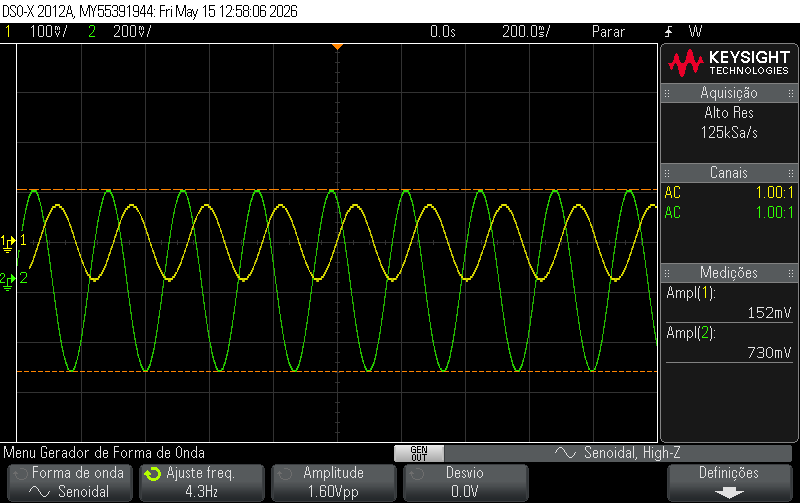
\includegraphics[width=\textwidth]{FIGURAS/4,3Hz_1.png} 
		\caption{Sinal na frequência de corte $f_1 = 4,3\text{ Hz}$ ($V_o \approx 730\text{ mV}$).}
		\label{fig:osc_f1}
	\end{minipage}
\end{figure}

% Grid 3: Osciloscópio - Banda de Rejeição
\begin{figure}[H]
	\centering
	\begin{minipage}{0.45\textwidth}
		\centering
		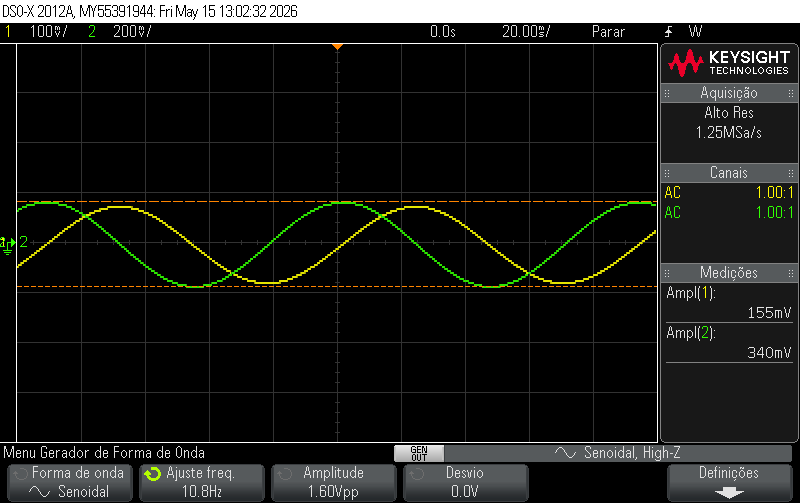
\includegraphics[width=\textwidth]{FIGURAS/10,8Hz_1.png} 
		\caption{Atenuação do sinal na frequência de $10,8\text{ Hz}$.}
		\label{fig:osc_10hz}
	\end{minipage}\hfill
	\begin{minipage}{0.45\textwidth}
		\centering
		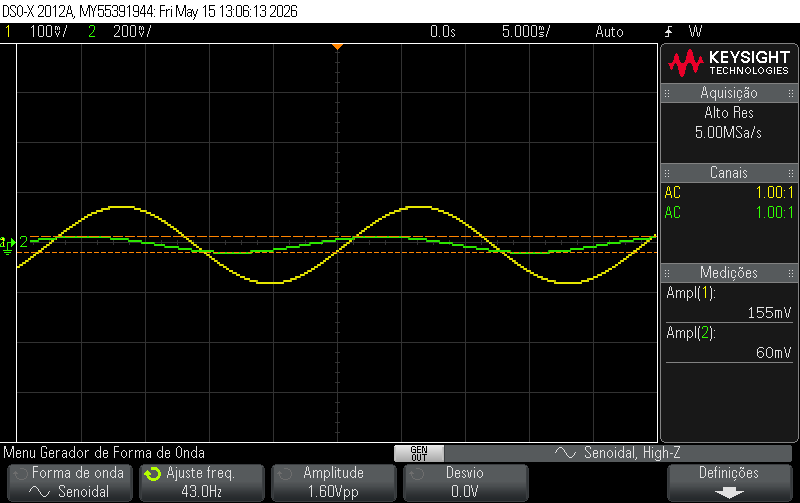
\includegraphics[width=\textwidth]{FIGURAS/43Hz_1.png} 
		\caption{Filtro em forte regime de atenuação na década posterior ($43,0\text{ Hz}$).}
		\label{fig:osc_43hz}
	\end{minipage}
\end{figure}


\section{Circuito 2: Filtro Passa-Baixa Subamortecido}

\subsection{Aferição a Frio dos Componentes Passivos}

De forma análoga ao procedimento adotado para o primeiro circuito, realizou-se a medição individual dos componentes passivos que constituem o Circuito 2. O intuito é registrar as discrepâncias introduzidas pela tolerância comercial, uma vez que a alteração dos resistores $R_1$ e $R_3$ modifica o sistema para um regime subamortecido, tornando-o altamente sensível a variações nos valores de capacitância e resistência. Os dados reais medidos encontram-se na Tabela \ref{tab:componentes_c2}.

\begin{table}[H]
	\centering
	\caption{Comparativo entre os valores nominais e medidos dos componentes - Circuito 2.}
	\label{tab:componentes_c2}
	\renewcommand{\arraystretch}{1.2}
	\begin{tabular}{ccc}
		\hline
		\textbf{Componente} & \textbf{Valor Nominal} & \textbf{Valor Medido Experimentalmente} \\ \hline
		Resistor $R_1$ & $470,0\text{ k}\Omega$ & $469,4\text{ k}\Omega$ \\
		Resistor $R_2$ & $470,0\text{ k}\Omega$ & $478,0\text{ k}\Omega$ \\
		Resistor $R_3$ & $47,0\text{ k}\Omega$ & $47,13\text{ k}\Omega$ \\
		Capacitor $C_1$ & $100,0\text{ nF}$ & $109,9\text{ nF}$ \\
		Capacitor $C_2$ & $10,0\text{ nF}$ & $11,42\text{ nF}$ \\ \hline
	\end{tabular}
\end{table}

\subsection{Determinação Prática da Frequência de Ressonância ($f_{max}$)}

Diferentemente do primeiro circuito, que é superamortecido e avaliado pela sua frequência de corte $f_1$, o Circuito 2 possui um comportamento subamortecido. Assim, o objetivo empírico principal foi localizar a frequência de ressonância ($f_{max}$), caracterizada por ser o ponto onde o ganho da função de transferência atinge o seu valor de pico máximo.

Configurou-se o gerador de sinais para fornecer uma onda senoidal com amplitude nominal de $5,0\text{ V}$. Monitorando os canais do osciloscópio, realizou-se uma varredura atenta nas frequências até observar o ponto de máxima excursão do sinal de saída. Verificou-se que a máxima transferência ocorreu com tensão de entrada a $5,0\text{ V}$ e a saída atingindo também cerca de $5,0\text{ V}$ a $5,1\text{ V}$. Nessas condições limítrofes, a frequência lida no osciloscópio foi de \textbf{$17,5\text{ Hz}$}. 

Este valor experimental de $f_{max} = 17,5\text{ Hz}$ é notavelmente consistente com as predições teóricas para este filtro, servindo como pivô para a varredura subsequente.

\subsection{Varredura de Frequência e Aquisição de Dados}

Com a frequência $f_{max} = 17,5\text{ Hz}$ estabelecida empíricamente, replicou-se o procedimento metodológico de medição aplicando fatores multiplicativos sobre $f_{max}$. Registrou-se a amplitude do sinal de entrada ($V_{in}$) e a amplitude atenuada do sinal de saída ($V_{out}$) para cada patamar. 

Os dados obtidos estão compilados na Tabela \ref{tab:varredura_c2}. Observa-se que a amplitude mantém-se estável próxima ao ganho unitário na banda de passagem e despenca de forma abrupta após o pico de ressonância ($f > 17,5\text{ Hz}$), validando o comportamento de atenuação rápida inerente a filtros de segunda ordem subamortecidos.

\begin{table}[H]
	\centering
	\caption{Dados experimentais de varredura de frequência para o Segundo Circuito ($f_{max} = 17,5\text{ Hz}$).}
	\label{tab:varredura_c2}
	\renewcommand{\arraystretch}{1.2}
	\begin{tabular}{cccc}
		\hline
		\textbf{Multiplicador} & \textbf{\textflorin  Calculada/Aplicada} & \textbf{Tensão de Entrada ($V_{in}$)} & \textbf{Tensão de Saída ($V_{out}$)} \\ \hline
		$0,15 \times f_{max}$ & $2,6\text{ Hz}$ & $4,7\text{ V}$ & $4,7\text{ V}$ \\
		$0,4 \times f_{max}$ & $7,0\text{ Hz}$ & $5,0\text{ V}$ & $5,0\text{ V}$ \\
		$0,6 \times f_{max}$ & $10,5\text{ Hz}$ & $5,0\text{ V}$ & $5,1\text{ V}$ \\
		$1,0 \times f_{max}$ & $17,5\text{ Hz}$ ($f_{max}$) & $5,0\text{ V}$ & $5,0\text{ V}$ \\
		$1,2 \times f_{max}$ & $21,0\text{ Hz}$ & $5,0\text{ V}$ & $4,7\text{ V}$ \\
		$1,4 \times f_{max}$ & $24,5\text{ Hz}$ & $5,0\text{ V}$ & $4,6\text{ V}$ \\
		$1,8 \times f_{max}$ & $31,0\text{ Hz}$ & $5,0\text{ V}$ & $3,9\text{ V}$ \\
		$2,5 \times f_{max}$ & $43,7\text{ Hz}$ & $5,0\text{ V}$ & $2,7\text{ V}$ \\
		$4,0 \times f_{max}$ & $70,0\text{ Hz}$ & $5,0\text{ V}$ & $1,3\text{ V}$ \\
		$6,0 \times f_{max}$ & $105,0\text{ Hz}$ & $5,0\text{ V}$ & $600\text{ mV}$ \\
		$10,0 \times f_{max}$ & $175,0\text{ Hz}$ & $5,1\text{ V}$ & $220\text{ mV}$ \\ \hline
	\end{tabular}
\end{table}

\subsection{Registro Fotográfico e Diagramático}

De modo a corroborar a fidelidade das informações anotadas em bancada, expõem-se as evidências visuais do Circuito 2. O arranjo em malha destaca o comportamento dos sinais sob as diferentes faixas de frequência exigidas pelo roteiro.

% Grid 1: Fotos da Montagem Física
\begin{figure}[H]
	\centering
	\begin{minipage}{0.45\textwidth}
		\centering
		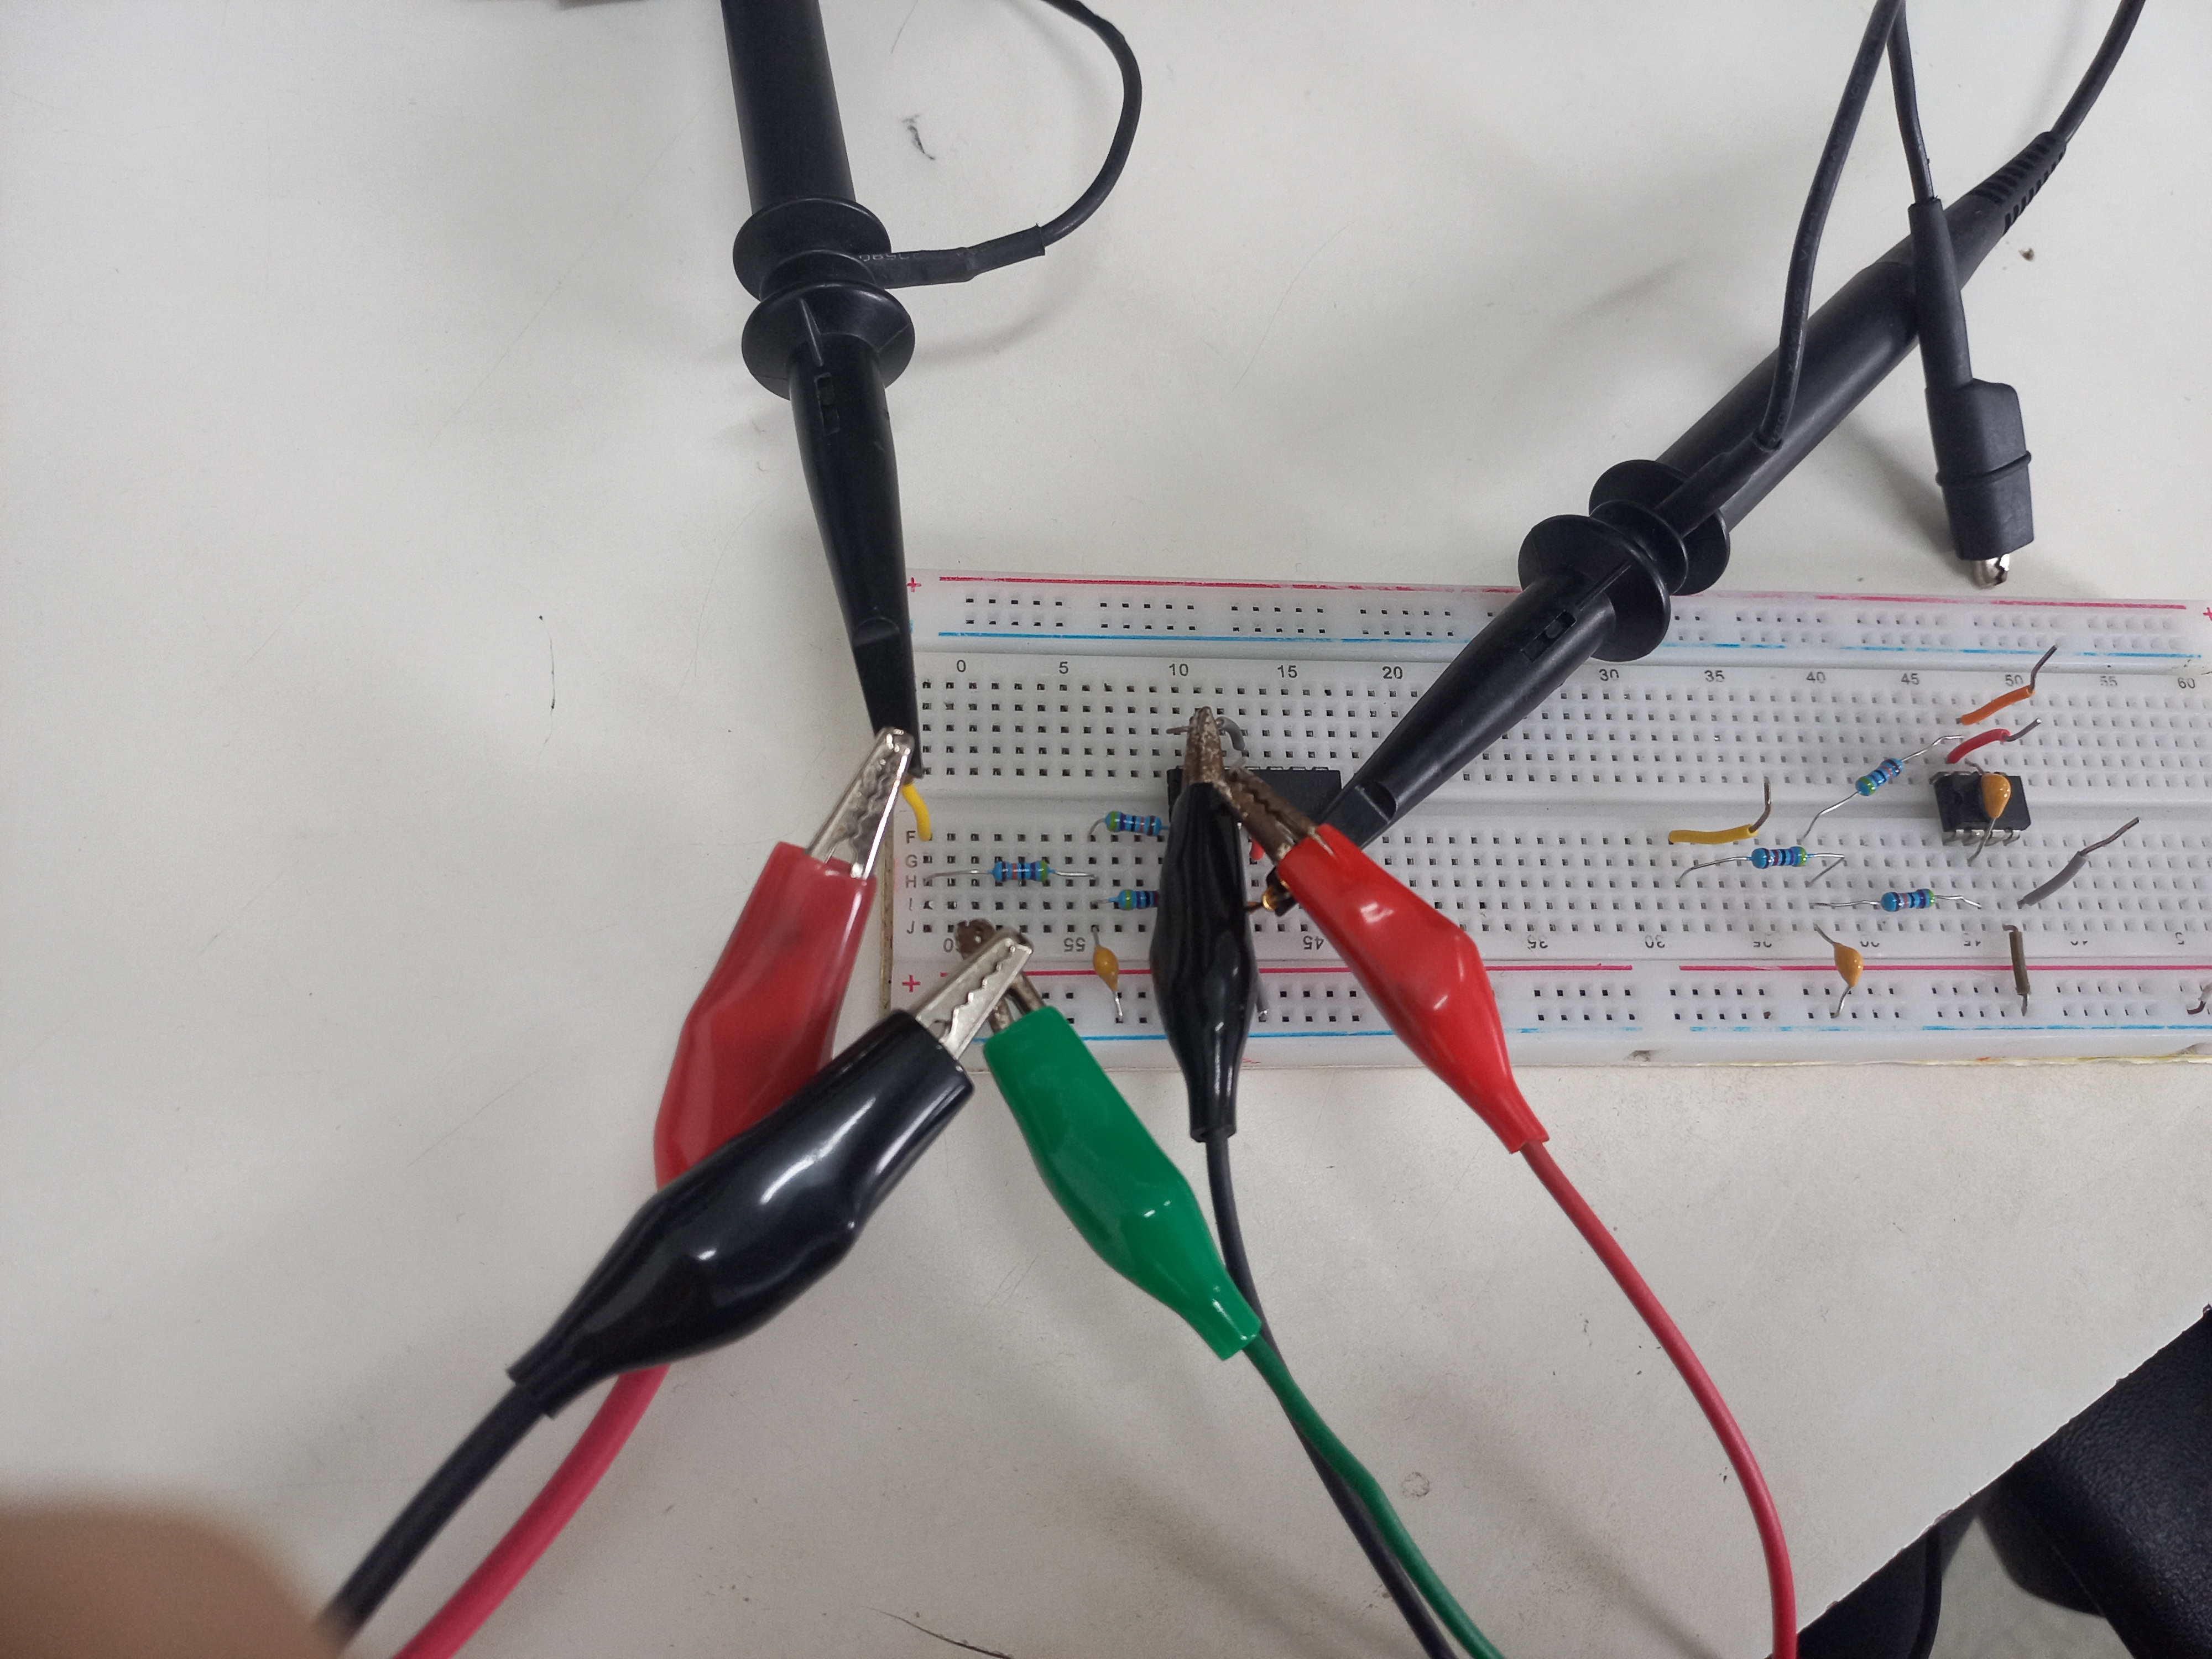
\includegraphics[width=\textwidth]{FIGURAS/circuito_2_montado.jpg}
		\caption{Vista lateral da configuração subamortecida (Circuito 2) montada na \textit{protoboard}.}
		\label{fig:c2_montado}
	\end{minipage}\hfill
	\begin{minipage}{0.45\textwidth}
		\centering
		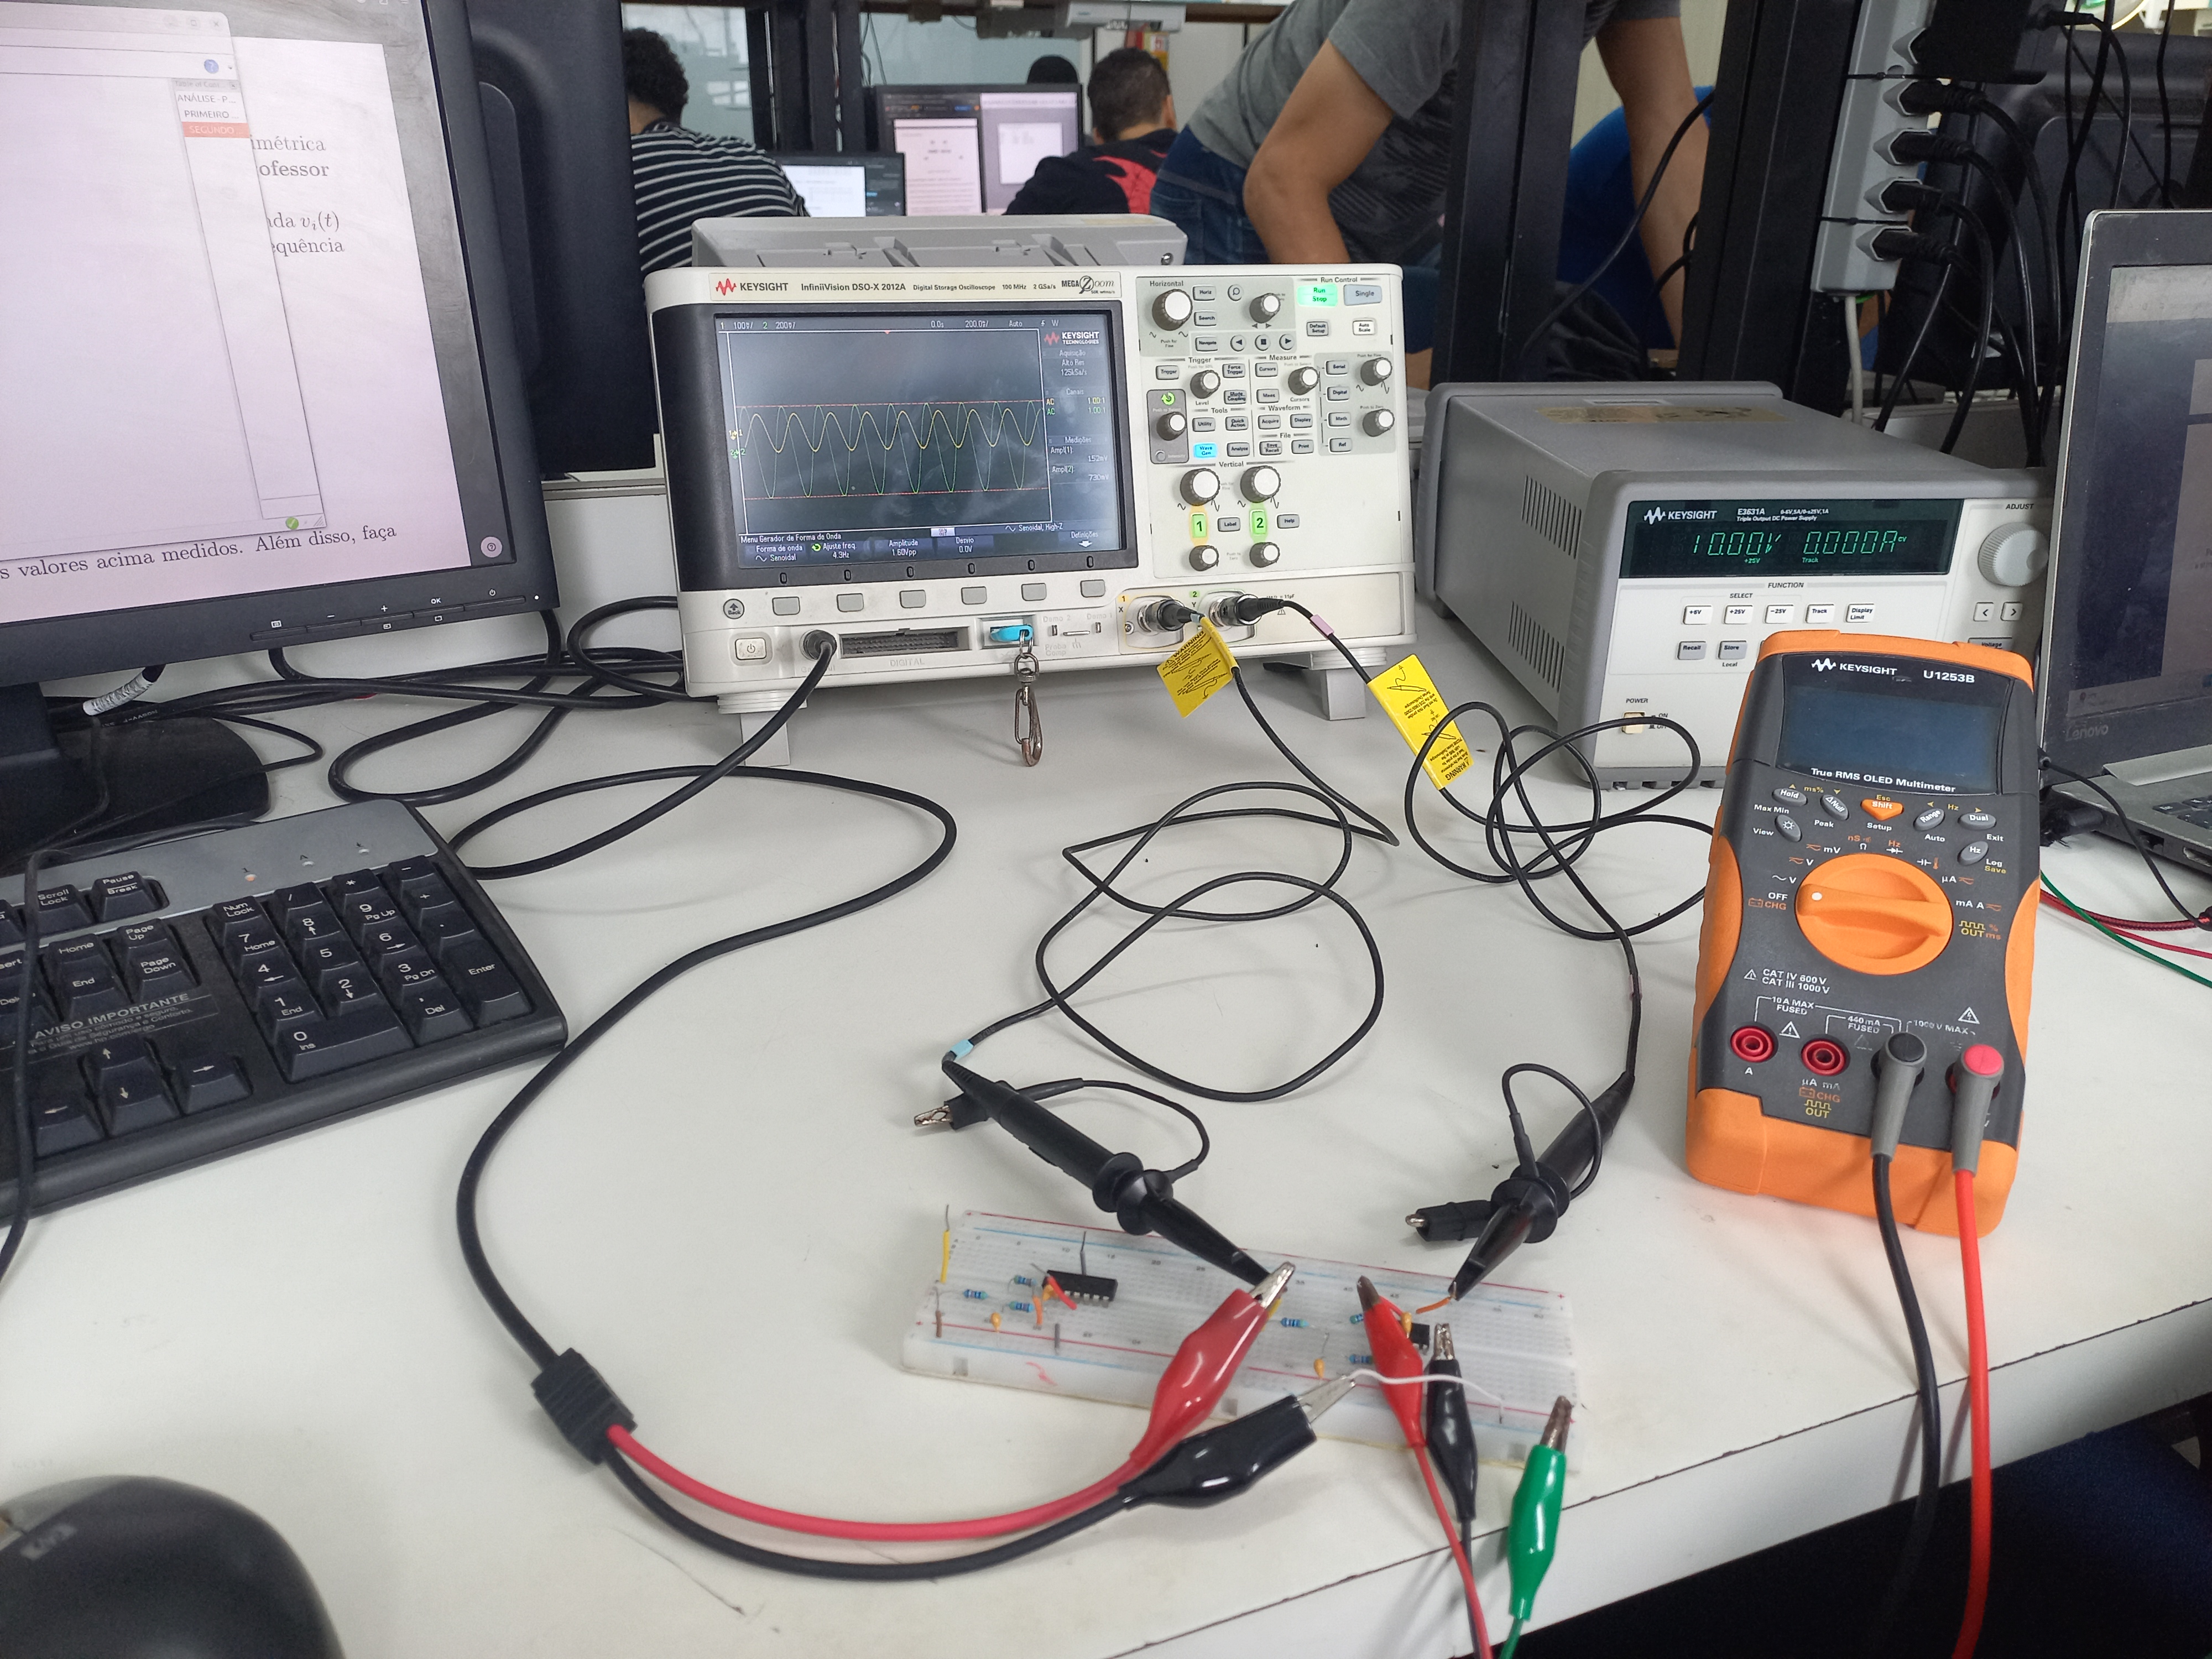
\includegraphics[width=\textwidth]{FIGURAS/bancada.jpg} 
		\caption{Perspectiva ampla dos equipamentos e da instrumentação durante os ensaios.}
		\label{fig:c2_bancada}
	\end{minipage}
\end{figure}

% Grid 2: Osciloscópio - Baixas Frequências e f_max
\begin{figure}[H]
	\centering
	\begin{minipage}{0.45\textwidth}
		\centering
		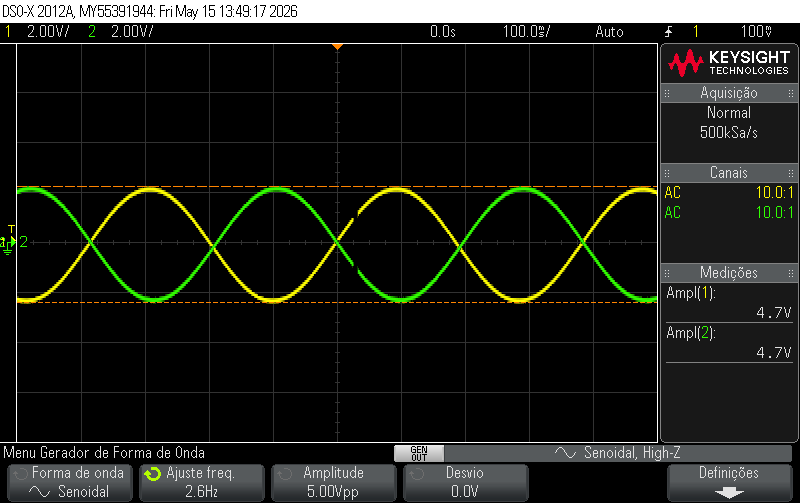
\includegraphics[width=\textwidth]{FIGURAS/2,6Hz_2.png} 
		\caption{Sinais a $2,6\text{ Hz}$, evidenciando o acoplamento de $V_{in}$ e $V_{out}$ na banda de passagem.}
		\label{fig:osc_2_6hz}
	\end{minipage}\hfill
	\begin{minipage}{0.45\textwidth}
		\centering
		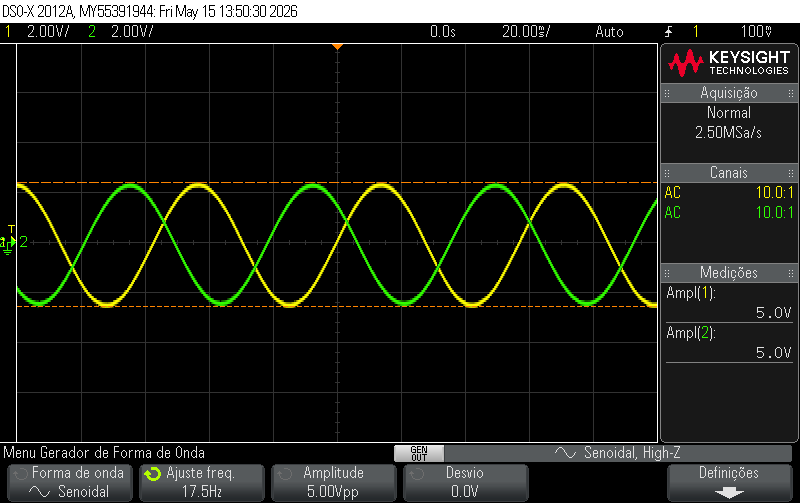
\includegraphics[width=\textwidth]{FIGURAS/17,5Hz_2.png} 
		\caption{Tensão de saída no ponto de ressonância $f_{max} = 17,5\text{ Hz}$.}
		\label{fig:osc_17_5hz}
	\end{minipage}
\end{figure}

% Grid 3: Osciloscópio - Banda de Rejeição
\begin{figure}[H]
	\centering
	\begin{minipage}{0.45\textwidth}
		\centering
		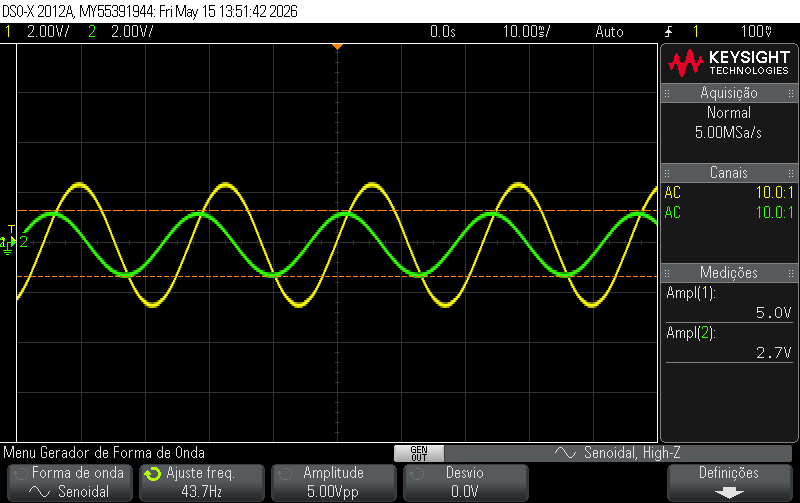
\includegraphics[width=\textwidth]{FIGURAS/43,7Hz_2.png} 
		\caption{Sinal sofrendo atenuação ($V_{out} = 2,7\text{ V}$) na frequência de $43,7\text{ Hz}$.}
		\label{fig:osc_43_7hz}
	\end{minipage}\hfill
	\begin{minipage}{0.45\textwidth}
		\centering
		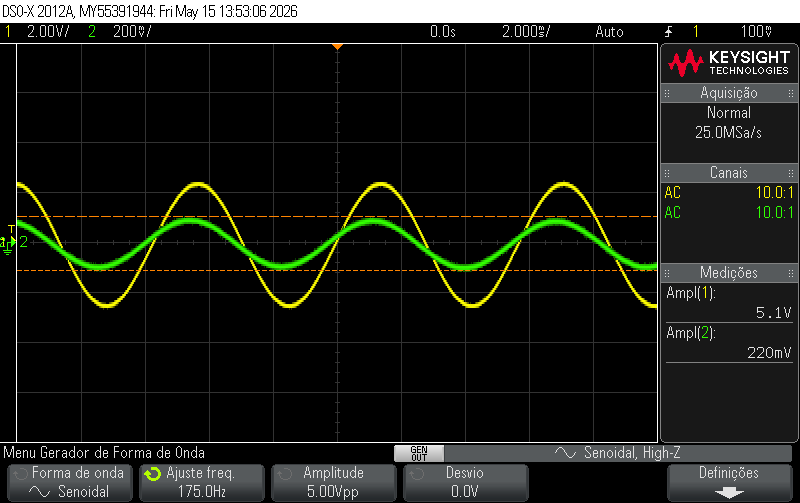
\includegraphics[width=\textwidth]{FIGURAS/175Hz_2.png} 
		\caption{Filtro em zona de corte profunda na década final ($175\text{ Hz}$), com $V_{out} = 220\text{ mV}$.}
		\label{fig:osc_175hz}
	\end{minipage}
\end{figure}

% -------------------------------------------------------------------------
% SEÇÃO DE INSTRUMENTAÇÃO
% -------------------------------------------------------------------------

\section{Instrumentação e Equipamentos Utilizados}

A confiabilidade das medições experimentais desta prática repousa fundamentalmente na precisão e calibração dos instrumentos de bancada empregados. Todo o procedimento laboratorial de excitação, leitura e diagnóstico dos parâmetros elétricos foi garantido por meio do seguinte \textit{setup} de alto desempenho:

\begin{itemize}
	\item \textbf{Multímetro Digital (True RMS):} Keysight U1253B. Utilizado primariamente para a medição ôhmica e capacitiva com alta acurácia (aferição a frio), atenuando incertezas paramétricas na análise de dados.
	\item \textbf{Fonte de Tensão Simétrica Contínua:} Keysight E3631A. Responsável pela polarização do amplificador operacional em $\pm 10\text{ V}$, garantindo baixos níveis de \textit{ripple} e ruído de linha acoplado.
	\item \textbf{Osciloscópio Digital (DSO):} Keysight DSO-X 2012A. Operado no modo de dois canais simultâneos, este equipamento possibilitou a leitura gráfica de pico a pico ($V_{pp}$) e a rápida constatação de defasagens e distorções dos sinais senoidais provenientes do gerador de funções.
\end{itemize}